%
% File acl2018.tex
%
%% Based on the style files for NAACL-HLT 2018, which were
%% Based on the style files for ACL-2015, with some improvements
%%  taken from the NAACL-2016 style
%% Based on the style files for ACL-2014, which were, in turn,
%% based on ACL-2013, ACL-2012, ACL-2011, ACL-2010, ACL-IJCNLP-2009,
%% EACL-2009, IJCNLP-2008...
%% Based on the style files for EACL 2006 by 
%%e.agirre@ehu.es or Sergi.Balari@uab.es
%% and that of ACL 08 by Joakim Nivre and Noah Smith

\documentclass[11pt,a4paper]{article}
\usepackage[hyperref]{acl2018}
\usepackage{times}
\usepackage{latexsym}
\usepackage{tikz}
\usetikzlibrary{positioning,shapes,shadows,arrows}


\usetikzlibrary{trees}
\usepackage{amsmath}
\usepackage{comment}
\usepackage{enumitem}
\usepackage{tabularx}
\usepackage{array}

\usepackage{booktabs}
\newcommand{\tabitem}{~~\llap{\textendash}~~}

\tikzstyle{every node}=[draw=black,thick,anchor=west,rounded corners,drop shadow,fill=white]
\tikzstyle{selected}=[draw=red,fill=red!30]
\tikzstyle{optional}=[dashed,fill=gray!50]

\newenvironment{tight_enumerate}{
\begin{enumerate}[leftmargin=4.0mm]
  \setlength{\itemsep}{0pt}
  \setlength{\parskip}{0pt}
}{\end{enumerate}}

\usepackage{url}

\aclfinalcopy % Uncomment this line for the final submission
%\def\aclpaperid{***} %  Enter the acl Paper ID here

\setlength\titlebox{7.5cm}
% You can expand the titlebox if you need extra space
% to show all the authors. Please do not make the titlebox
% smaller than 5cm (the original size); we will check this
% in the camera-ready version and ask you to change it back.

\newcommand\BibTeX{B{\sc ib}\TeX}

% bcw 2/20: suggest different title
%\title{A Detailed Hierarchical Corpus for Modeling Medical Literature}
%\title{A New Corpus for NLP in Evidence-Based Medicine}
\title{A Corpus with Multi-Level Annotations of Patients, Interventions and Outcomes to Support Language Processing for Medical Literature}
% bcw 2/21 -- i like this title, but i'm not sure we won't to imply this is *only* good for medical search? i think, e.g., being able to pick out structured PICO elements, study design attributes, etc., has potential use beyond search (although certainly useful for that). 
% Jessy 2/21 ...to support language processing in medical literature?
% bcw 2/22 -- i like that! have changed for now -- @Ani let me know if you disagree?

% bcw 5/10 TODO add authors & affiliations!
%\authot{Ben, Jessy, Roma, Yinfei, Ian, Ani, Byron}
% bcw 5/11 -- added but it doesn't look great... open to better formatting options
\author{Benjamin Nye \\
  Northeastern University \\
  {\small\tt nye.b@husky.neu.edu}  \\\And 
  Junyi Jessy Li \\ 
  UT Austin \\ 
  {\small\tt jessy@austin.utexas.edu} \\\And
  Roma Patel \\
  Rutgers University\\
  {\small\tt romapatel996@gmail.com} \\\AND
  Yinfei Yang\thanks{* now at Google Inc.} \\
  \emph{No affiliation} \\
  {\small\tt yangyin7@gmail.com} \\ \\\And 
  Iain J. Marshall \\
  King's College London \\
  {\small\tt iain.marshall@kcl.ac.uk} \\\And
  Ani Nenkova \\
  UPenn \\
  {\small\tt nenkova@seas.upenn.edu} \\\AND
  Byron C. Wallace \\
  Northeastern University \\
  {\small\tt b.wallace@northeastern.edu}}
  
\date{}

\begin{document}
\maketitle
\begin{abstract}

% bcw 2/21 -- obviously too long, sorry.
% bcw 2/21 -- update: now only probably too long, after cutting. 
We present a corpus of 5,000 richly annotated abstracts of medical articles describing %the conduct and results of 
clinical randomized controlled trials. Annotations include demarcations of text spans that describe the Patient population enrolled, the Interventions studied and to what they were Compared, and the Outcomes measured (the `PICO' elements). These spans are further annotated at a more granular level, e.g., individual interventions within them are marked and mapped onto a structured medical vocabulary. We acquired annotations from a diverse set of workers with varying levels of expertise and cost. We describe our data collection process and the corpus itself in detail. We then outline a set of challenging NLP tasks that would aid searching of the medical literature and the practice of evidence-based medicine. 
%ANI removed emphasis above. Looks odd in the abstract
%ANI the baselines are a part of the outline of the task, I have removed the sentence below; also let's not say we want to encourage people to do stuff, it is implied in the setting up of a challenging task :)
%Using the corpus we introduce, we present a set of baseline models and results for these tasks. We hope to encourage other NLP researchers to work in this important domain.
%(and provide associated baseline models and results) made possible by this corpus  motivated by the domain of Evidence-Based Medicine generally and this dataset in particular. % Our hope is to motivate NLP researchers to work on this stuff ... % bcw 2/20 maybe conclude w/something ra-ra like this??
% Repeated mentions of particular PICO elements were also marked as such.
\end{abstract}

%%%
% bcw, meta aims:
% 1. EBM 
% 2. the need for corpora in this space
\section{Introduction}
\label{section:intro}
 
%For decades, the relentless growth of the biomedical literature has posed a serious challenge to domain experts attempting to synthesize the knowledge pertaining to a particular topic \cite{bastian2010seventy}. For example, 
In 2015 alone, about 100 manuscripts describing randomized controlled trials (RCTs) for medical interventions were published \emph{every day}. It is thus practically impossible for physicians to know which is the best medical intervention for a given patient group and condition  \cite{borah2017analysis,fraser2010impossibility,bastian2010seventy}.
%, as this would require wading through unstructured texts to gather all reported results. 
This inability to easily search and organize the published literature impedes the aims of \emph{evidence based medicine} (EBM), which aspires to inform patient care using the totality of %available 
relevant evidence. % EBM relies on experts to efficiently retrieve and synthesize large sets of relevant documents. %collect and parse a large number of relevant documents.
% This process is both expensive and time consuming \citep{allen1999estimating,borah2017analysis}. This makes it difficult to keep evidence syntheses up-to-date, which in turn hinders the practice of evidence based care. 
% bcw 2/20: @TODO I/we should say more below about the specific NLP tasks, people will want to know this upfront. 
% bcw 2/22 hmmm maybe don't need this para but feel like need to transition from EBM -> NLP
Computational methods could expedite biomedical evidence synthesis \cite{tsafnat2013automation,wallace2013modernizing} and natural language processing (NLP) in particular can play a key role in the task. 
%helping domain experts search, extract data from, and synthesize the findings reported in published reports of clinical trials. 
%The medical domain poses clear challenges from an NLP vantage point, including processing technical language and identifying and disambiguating clinical `entities' such as interventions and outcomes). EBM thus provides an ideal domain for NLP research, in that it motivates methodological challenges that, if solved, would yield considerable practical impact in medicine. 
%The domain of EBM thus constitutes an ideal scenario in which work on methods to address the core technical issues may realize a considerable practical impact in medicine. 

%Recognizing this potential, there have been some efforts toward automating evidence synthesis using NLP. 

Prior work has explored the use of NLP methods to automate biomedical evidence extraction and synthesis \cite{boudin2010positional,marshall:2017:ACL,ferracane2016leveraging,verbeke2012statistical}.\footnote{There is even, perhaps inevitably, a systematic review of such approaches \cite{jonnalagadda2015automating}.} But the area has attracted less attention than it might from the NLP community, due primarily to a dearth of publicly available, annotated corpora with which to train and evaluate models. %We address this gap by providing a resource to facilitate work on NLP for EBM.  

% bcw 2/19 -- i think we need a catchy corpus name?
% bcw 2/19 -- for website below we need to pull everything together into a neat format for browsing/download. 
% bcw 2/22 -- re: catchy name -- maybe "EBMNLP"? almost like "EMNLP"... maybe *too* close... 
% Jessy 2/22: How about EBMLP? :)))
% bcw 5/10 TODO actually create the website for the corpus ! I'm fine to host it at a different URL, too; whatever is easiest and we are confident we can maintain indefinitely (can also always redirect)
% bcw 5/11 -- have updated to Ben's proposed URL :)
Here we address this gap by introducing \emph{EBM-NLP}, a new corpus to power NLP models in support of EBM. The corpus, accompanying documentation, baseline model implementations for the proposed tasks, and all code are publicly available.\footnote{\url{http://www.ccs.neu.edu/home/bennye/EBM-NLP}} EBM-NLP comprises $\sim$5,000 medical abstracts describing clinical trials, multiply annotated in detail with respect to characteristics of the underlying trial Populations (e.g., \emph{diabetics}), Interventions (\emph{insulin}), Comparators (\emph{placebo}) and Outcomes (\emph{blood glucose levels}). Collectively, these key informational pieces are referred to as PICO elements; they form the basis for well-formed clinical questions \cite{huang2006evaluation}. % bcw 2/22 this is a actually maybe a sort of weird paper to cite tos upport this, since that paper is a little bit critical of PICO for QA, but on the other hand they end up concluding that it's the best we've got basically, so i dunno

%Relying exclusively on medical doctors (MDs) to provide annotations would be prohibitively expensive. Therefore, 
We adopt a hybrid crowdsourced labeling strategy using heterogeneous annotators with varying expertise and cost, from laypersons to MDs. Annotators were first tasked with marking text spans that described the respective PICO elements. Identified spans were subsequently annotated in greater detail: this entailed finer-grained labeling of PICO elements and mapping these onto a normalized vocabulary, and indicating redundancy in the mentions of PICO elements. 

In addition, we outline several NLP tasks that would directly support the practice of EBM and that may be explored using the introduced resource. We present baseline models and associated results for these tasks. 

%. For example, in this phase, labelers marked sub-spans pertaining to individual interventions and outcomes; mapped spans onto a normalized, publicly available biomedical vocabulary (MeSH); identified and tagged structured data such as sample sizes; and indicated when PICO elements were discussed redundantly.
%(e.g., by marking sub-spans referencing the same intervention).  

% bcw 2/20 -- too long too long i know
%Our contributions are summarized as follows. (1) we present a new, relatively large (for this domain) publicly available corpus of richly annotated biomedical abstracts to facilitate NLP work in this space. (2) We formalize key NLP tasks that would support evidence extraction (and thus EBM) and provide baseline models and results for these.  (3) Our data collection process (in which we rely on a heterogeneous annotators, from laypersons to MDs) provides insights into strategies for constructing NLP corpora in specialized domains.
%This addresses a major hindrance of NLP researchers hoping to work on important medical tasks: a dearth of readily available corpora. Our hope is that this dataset is used to build novel models that aid specialists attempting to make sense of the biomedical evidence base.

\begin{comment}
\begin{itemize}
\item We present a new, high-quality, publicly available corpus of richly annotated biomedical abstracts. This addresses a major hindrance of NLP researchers hoping to work on important medical tasks: a dearth of readily available corpora. Our hope is that this dataset is used to build novel models that aid specialists attempting to make sense of the biomedical evidence base.

\item Annotating biomedical abstracts constitutes a difficult task, but relying exclusively on MDs would be prohibitively expensive. The approach we outline in this work provides evidence that hybrid crowdsourced strategies can be used to build relatively high-quality corpora, even in specialized domains.
\end{itemize}
\end{comment}

% bcw 2/20 -- even though i've included it here, i don't usually like ToC mini-paragraphs like this, but felt for whatever reason like it was more useful / needed for this kind of paper.
% Jessy 2/21: if you think this is adding too much length, maybe possibly merge with the previous contribution paragraph (and after each contribution, specify which sections)?
%The remainder of this paper is structured as follows. We review existing resources and related work (Section \ref{section:related-work}). Then we describe our annotation schema and data collection process (Section \ref{section:collection}). We provide basic statistics characterizing the derived corpus in Section \ref{section:the-corpus}. In Section \ref{section:tasks-baselines} we outline several NLP tasks that would directly support the practice of EBM and that may be explored using the presented resource. We also outline baseline models and results for these tasks. 

%Recent work has provided some relief in the form of tools and techniques to aide researchers (TODO: cite roboreviewer, mesh search strategies).

% bcw 12/14: this is a super important issue, but seems tangential to our aims here no? this might speak more to better searchability of *reviews* rather than *primary literature*? Although, the dream would be to simply have models that can assemble synthese on demand, obviating the need for Cochrane in the first place... but I digress
%Despite concerted efforts from groups such as the Cochrane Collaboration to create and disseminate high quality systematic reviews (SRs), uptake by medical practitioners remains low.
%Only 5\% of surveyed doctors reported frequently consulting SRs \cite{thor2016design}.
%While initiatives in education and training help combat this issue, a lack of confidence in the searchability of the literature presents a significant barrier to the adoption of EBM practices \citep{mcalister1999evidence}.




\section{Related Work}
\label{section:related-work}

We briefly review two lines of research relevant to the current effort: work on NLP to facilitate EBM, and research in crowdsourcing for NLP. 

%\paragraph*{NLP for EBM}
% bcw 2/22 -- literally just adding subsection back because we have some space to fill... 
\subsection{NLP for EBM}
Prior work on NLP for EBM has been limited by the availability of only small corpora, which have typically provided on the order of a couple hundred annotated abstracts or articles for very complex information extraction tasks. For example, the ExaCT system \cite{kiritchenko2010exact} applies rules to extract 21 aspects of the reported trial. It was developed and validated on a dataset of 182 marked full-text articles. The ACRES system \cite{summerscales2011automatic} produces summaries of several trial characteristic, and was %extracted from the abstract 
trained on 263 annotated abstracts.
%Two previously developed efforts to build NLP systems to extract data from medical literature are ExaCT \cite{kiritchenko2010exact} and ACRES \cite{summerscales2011automatic}. Both efforts developed corpora that is now publicly available. The corpus released with ExaCT comprises HTML/XML articles \cite{kiritchenko2010exact}. ACRES ingests abstracts and from these produces summaries of extracted variables. Both corpora are modest in size: the former includes 182 marked full-text articles, while the latter comprises 263 annotated abstracts. 
% Jessy 2/21: not sure if you want to cite this, but there's a short paper on sentence classification for PICO at EACL 2017: http://aclweb.org/anthology/E17-2110
% bcw 2/22: cool pointer Jessy! but not PICO specifically as far as I can tell. still looks interesting!
% bcw 2/20: this can definitely be cut down.
% bcw 2/22: ok dropped the dtails basically
Hinting at more challenging tasks that can build upon foundational information extraction, Alamri and Stevenson \shortcite{alamri2015automatic} developed methods for detecting contradictory claims in biomedical papers. Their corpus of annotated claims contains 259 sentences \cite{alamri2016corpus}.


%More recent related work due to Alamri and Stevenson \cite{alamri2015automatic} entailed developing NLP models for detecting contradictory claims in biomedical papers. For this they developed a small corpus comprising claims in 259 sentences \cite{alamri2016corpus}. % They consider triplets comprising a proposition $F$ and two sentences $S_1$, $S_2$; the idea is infer whether $S_1$ agrees with or contradicts $S_2$ with respect to $F$. They assembled a small corpus by collecting abstracts of clinical trials  and tasking an expert to generate binary (\emph{yes}/\emph{no}) propositions that could be answered based on the abstract. They acquired such annotations on claims identified in 259 sentences \cite{alamri2016corpus}. 


%The corpus
% bcw: for exact, i get the 182 from 132 train + 50 for test set: https://bmcmedinformdecismak.biomedcentral.com/articles/10.1186/1472-6947-10-56#Sec2

%The available datasets just reviewed are annotation rich, but small in size. 
Larger corpora for EBM tasks have been derived using (noisy) automated annotation approaches. This approach has been used to build, e.g., datasets to facilitate work on Information Retrieval (IR) models for biomedical texts 
\cite{scells2017test,chung2009sentence,boudin2010positional}. Similar approaches have been used to `distantly supervise' annotation of full-text articles describing clinical trials \cite{wallace2016extracting}. In contrast to the corpora discussed above, these automatically derived datasets tend to be relatively large, but they include only shallow annotations.


%e.g., 
%via `distant supervision' 
% Existing resources for medical text tend to fall in to one of two categories: feature-rich but limited in size \citep{chung2009sentence,summerscales2011automatic}, or very large but lacking detailed word-level annotations (TODO: cite medline, Byron's distant supervision). % bcw 12/14 also need to cite summerscales older stuff and mark stevenson's recent stuff on NLI type annotations/models for RCTs

%In contrast to existing resources, in this work we set out to develop a new, publicly available corpus that is both richly annotated and relatively large. 

%We acquired detailed, hierarchical token-wise annotations corresponding to study PICO elements. One reason that such a corpus has not yet been developed is cost: properly trained healthcare professionals (MDs) are time-constrained and (often prohibitively) expensive. We address this by adopting a hybrid crowd-sourcing approach to labeling, enlisting a diverse set of annotators with a mix of costs and expertise levels. 


Other work attempts to bypass basic extraction tasks and address more complex biomedical QA and (multi-document) summarization problems to support EBM \cite{demner2007answering,molla2011development,abacha2015means}. Such systems would directly benefit from more accurate extraction of the types %of structured data 
codified in the corpus we present here.
%, i.e., the data and tasks we present are likely to improve downstream QA and summarization systems. 

% bcw 2/22 -- maybe not necessary to have separate subsection but felt otherwise felt a bit odd mixed in w/above... 
% also there are two topics here, crowdsourcing generally then crowdsourcing in NLP
%\paragraph*{Crowdsourcing}% to build NLP corpora}

% bcw 2/22 -- again, just eating some space -- the reverse of what we usually have to do!
\subsection{Crowdsourcing}

%%% need to mention cochrane crowd
% TODO just want one para mentioning that this is feasible
Crowdsourcing, which we here define operationally as the use of distributed lay annotators, has shown encouraging results in NLP \cite{novotney2010cheap,sabou2012crowdsourcing}. Such annotations are typically imperfect, but methods that aggregate redundant annotations can mitigate this problem \cite{dalvi2013aggregating,hovy2014experiments,nguyen2017aggregating}.

Medical articles contain relatively technical content, which intuitively may be difficult for persons without domain expertise to annotate. However, recent promising preliminary work has found that crowdsourced approaches can yield surprisingly high-quality annotations in the domain of EBM specifically \cite{mortensen2017exploration,thomas2017living,wallace2017identifying}. 


% bcw 2/22 -- this should go elsewhere, not related work
%In addition to the crowd-sourced annotations, we collected expert annotations from medical students and doctors on a small subset of documents to provide a set of high quality labels to use for dataset validation.





\section{Data Collection}
\label{section:collection}

\begin{figure*}
\centering
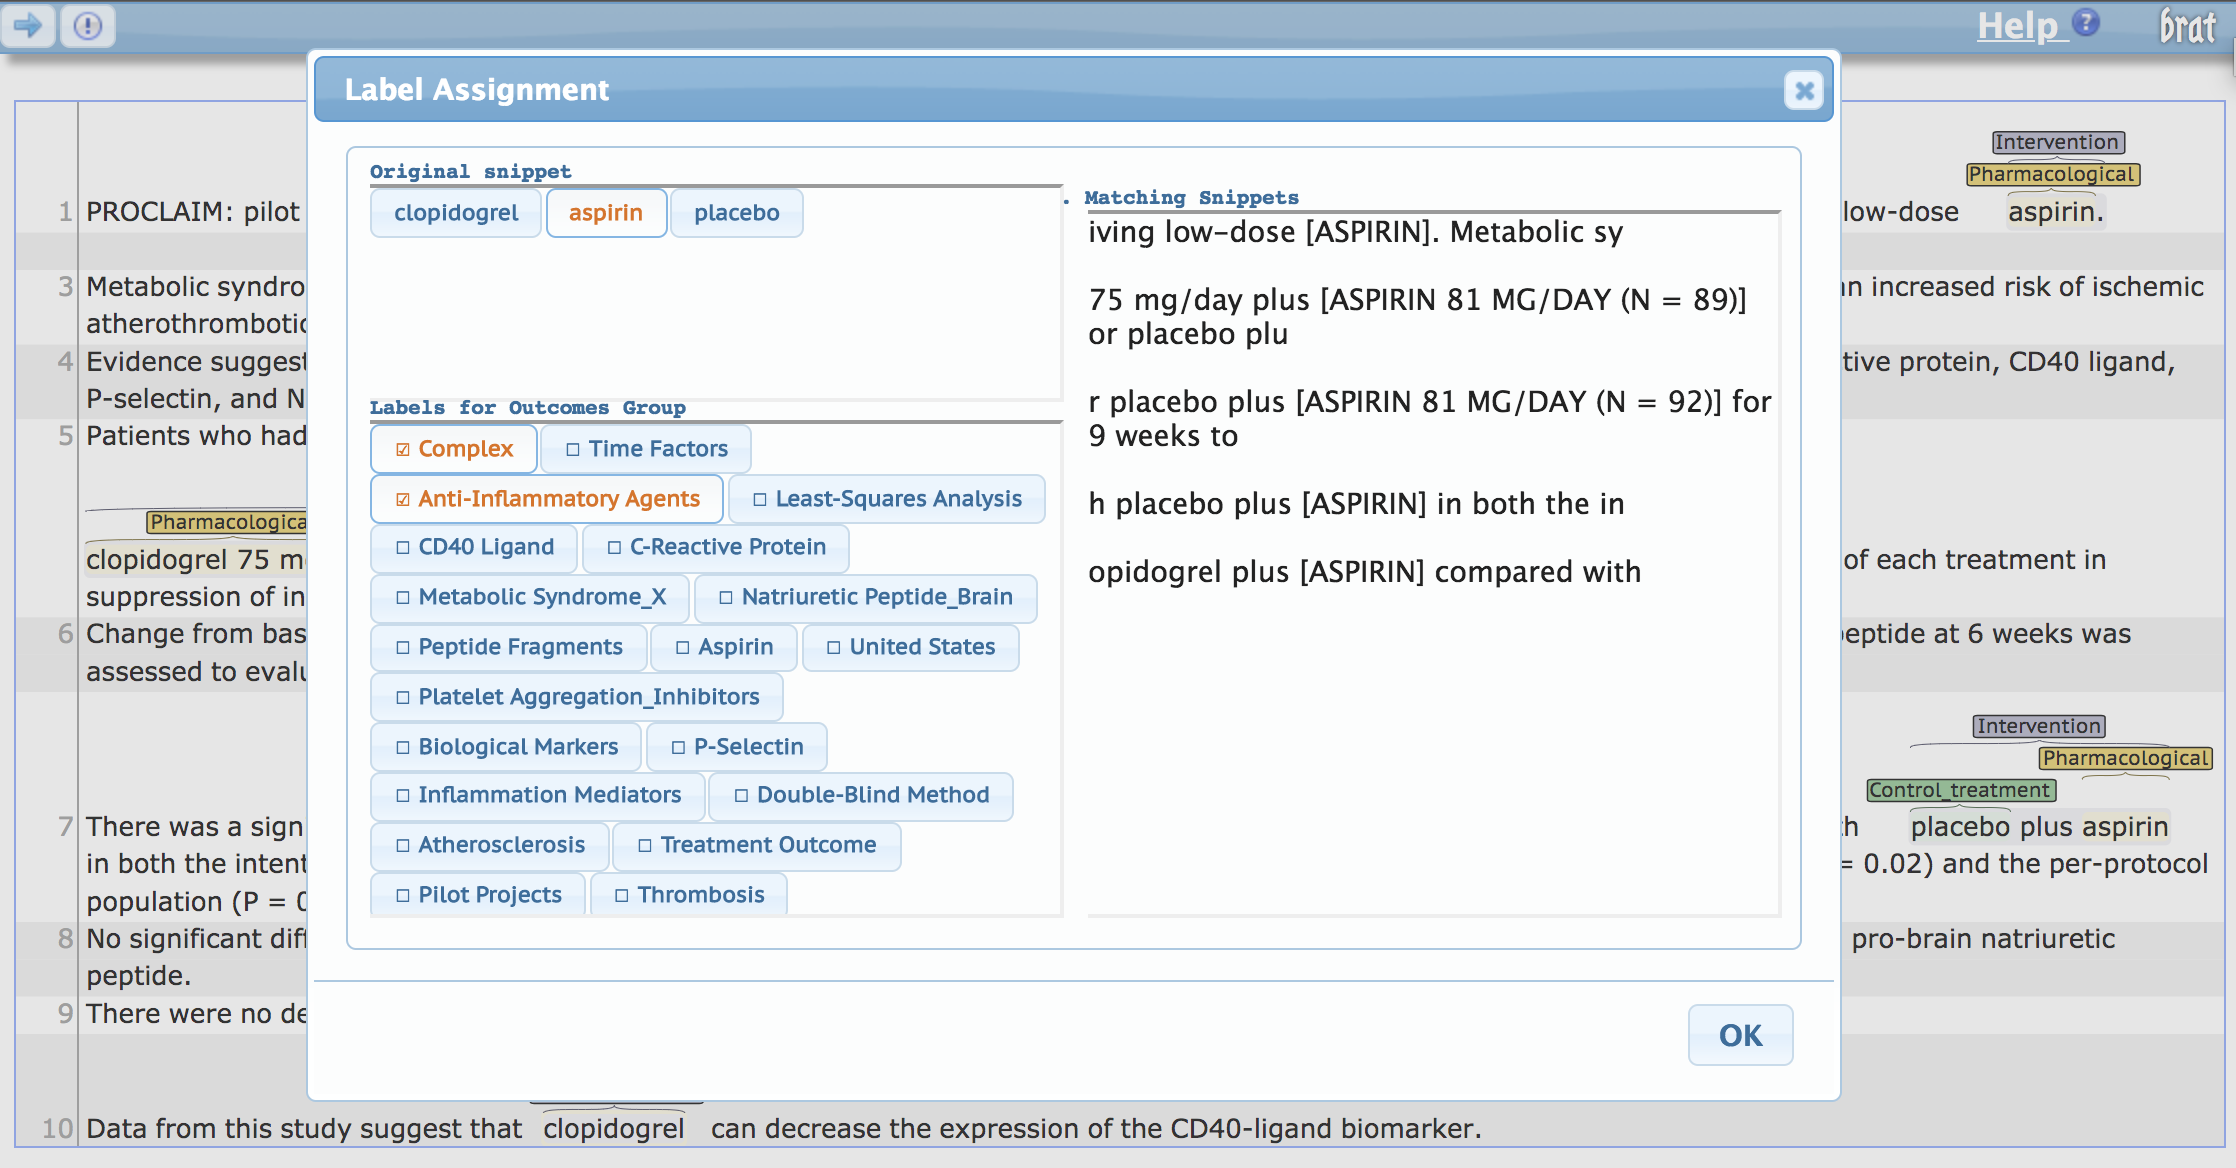
\includegraphics[width=0.8\linewidth]{figs/mesh_interface}
\caption{Annotation interface for assigning MeSH terms to snippets.}
\end{figure*}

% bcw 2/20 -- not clear to me what this meant? 
%   "and a set of tags categorizing the contents"

% bcw 2/20 -- be sure not to conflate MEDLINE articles with RCTs; the majority of studies in MELDINE are not trials
% bcw 2/20 -- excellent use of 'bevy'!
% ANI Really? My dictionary says its an informal word and I did need to look it up :)
% bcw 5/10 : I stand by my assessment :) formality be damned!
PubMed provides access to the MEDLINE database\footnote{\url{https://www.nlm.nih.gov/bsd/pmresources.html}} which indexes titles, abstracts and meta-data for articles from selected medical journals dating back to the 1970s. MEDLINE indexes over 24 million abstracts; the majority of these have been manually assigned metadata which we used to retrieved a set of 5,000 articles describing RCTs with an emphasis on cardiovascular diseases, cancer, and autism. These particular topics were selected to cover a range of common conditions.

%annotated with a bevy of fields. In the case of articles describing clinical trials, these fields code for properties of the study. We retrieved a set of 5,000 articles from the set of Randomized Controlled Trials (RCTs) indexed on MEDLINE by sampling from the set of all RCTs with an emphasis on cardiovascular diseases, cancer, and autism. These particular topics were selected to cover a range of common conditions. 
% bcw 2/22: @IAIN this seem ok? 

% TODO: details about MeSH tag process?

We decomposed the annotation process into two steps, performed in sequence. First, we acquired labels demarcating spans in the text describing the clinically salient abstract elements mentioned above: the trial Population, the Interventions and Comparators studied, and the Outcomes measured. We collapse Interventions and Comparators into a single category (I).
In the second annotation step, we tasked workers with providing more granular (sub-span) annotations on these spans. 

For each PIO element, all abstracts were annotated with the following four types of information.
% TODO: need explanation of PICO elements?
%\begin{tight_enumerate}%[itemsep=-1ex]
\begin{enumerate}
\item \textbf{Spans} exhaustive marking of text spans containing information relevant to the respective PIO categories (Stage 1 annotation).
\item \textbf{Hierarchical labels} assignment of more specific labels to subsequences comprising the marked relevant spans (Stage 2 annotation).
\item \textbf{Repetition} grouping of labeled tokens to indicate repeated occurrences of the same information (Stage 2 annotation).
\item \textbf{MeSH terms} assignment of the metadata MeSH terms associated with the abstract to labeled subsequences (Stage 2 annotation).\footnote{MeSH is a controlled, structured medical vocabulary maintained by the National Library of Medicine.}   % bcw 2/20 -- i do not think we have explained MeSH at this point??
% Jessy 2/21: there is one sentence in the intro, but a refresher here will be good.
\end{enumerate}
%\end{tight_enumerate}

We collected annotations for each P, I and O element individually to avoid the cognitive load imposed by switching between label sets, and to reduce the amount of instruction required to begin the task. All annotation was performed using a modified version of the Brat Rapid Annotation Tool (BRAT) \citep{stenetorp2012brat}. We include all annotation instructions provided to workers for all tasks in the Appendix.

%, which places an emphasis on an intuitive interface and accessibility to non-technical users .


\subsection{Non-Expert (Layperson) Workers}

For large scale crowdsourcing via recruitment of layperson annotators, we used Amazon Mechanical Turk (AMT). All workers were required to have an overall job approval rate of at least 90\%. Each job presented to the workers required the annotation of three randomly selected abstracts from our pool of documents. As we received initial results, we blocked workers who were clearly not following instructions, and we actively recruited the best workers to continue working on our task at a higher pay rate. 

We began by collecting the least technical annotations, moving on to more difficult tasks only after restricting our pool of workers to those with a demonstrated aptitude for the jobs. We obtained annotations from $\geq 3$ different workers for each of the 5,000 abstracts to enable robust inference of reliable labels from noisy data. After performing filtering passes to remove non-RCT documents or those missing relevant data for the second annotation task, we are left with between 4,000 and 5,000 sets of annotations for each PIO element after the second phase of annotation. % bcw 5/10 TODO need to note that we end up w/less than 5k, due to various reasons including filtering out non-RCTs

\subsection{Expert Workers}

To supplement our larger-scale data collection via AMT, we collected annotations for 200 abstracts for each PIO element from workers with advanced medical training. The idea is for these to serve as reference annotations, i.e., a test set with which to evaluate developed NLP systems. We plan to enlarge this test set in the near future, at which point we will update the website accordingly. % bcw 5/10 adding this note

% bcw/22: below was: "University of Pennsylvania and Drexel University"  
% bcw 5/10 -- added back in
For the initial span labeling task, two medical students from the University of Pennsylvania and Drexel University provided the reference labels. % Jessy 2/21: is this revealing for double-blind review? (really not sure so just checking). % bcw 2/22 -- good catch, let's be safe
In addition, for both stages of annotation and for the detailed subspan annotation in Stage 2, we hired three medical professionals via Upwork,\footnote{\url{http://www.upwork.com}} an online platform for hiring skilled freelancers. %and provides detailed bibliographic information about potential workers.
After reviewing several dozen suggested profiles, we selected three workers that had the following characteristics: Advanced medical training (the majority of hired workers were Medical Doctors, the one exception being a fourth-year medical student); Strong technical reading and writing skills; And an interest in medical research. % bcw 2/20 -- is it correct to say they all had MDs???  i mean students clearly don't i realize, but all upworkers?
% ben 2/21 -- Mohamed is a a 4th year med student I believe, so not an MD yet
In addition to providing high-quality annotations, individuals hired via Upwork also provided feedback regarding the instructions to help make the task as clear as possible for the AMT workers.



\begin{comment}
\begin{tight_enumerate}%[itemsep=-1ex]
\item Advanced medical training
\item Strong technical reading and writing skills
\item An interest in medical research
\end{tight_enumerate}
\end{comment}


\section{The Corpus}
\label{section:the-corpus}

% bcw 2/22 -- can probably go if we need the space but wanted to orient the reader a bit 
We now present corpus details, paying special attention to worker performance and agreement. We discuss and present statistics for acquired annotations on spans, tokens, repetition and MeSH terms in Sections \ref{section:corpus-spans}, \ref{section:corpus-tokens}, \ref{section:corpus-coref}, and \ref{section:corpus-mesh}, respectively.

\begin{table*} % ben 2/22 -- my latex-fu is weak and this is as reasonable as I could get it looking % bcw 2/22 -- i think it's great.
\centering
\small
\begin{tabularx}{\linewidth}{ m{0.1cm} m{2.6cm} l X }
%\hline
\noalign{\vskip 1mm}  
\multicolumn{4}{l}{\textbf{P} \emph{Fourteen children (12 infantile autism full syndrome present, 2 atypical pervasive developmental disorder) between 5 and}} \\
\multicolumn{4}{l}{\emph{13 years of age}} \\
\noalign{\vskip 1mm}  

& Text & Label & MeSH terms \\
\cline{2-4}
\noalign{\vskip 1mm}  
& \tabitem Fourteen & \textsc{Sample Size (full)}    & \\
& \tabitem children & \textsc{Age (young)}              & \\
& \tabitem 12       & \textsc{Sample Size (partial)} & \\
& \tabitem autism   & \textsc{Condition (disease)}   & Autistic Disorder, Child Development Disorders Pervasive \\
& \tabitem 2        & \textsc{Sample Size (partial)} & \\
& \tabitem 5 and 13 & \textsc{Age (young)}             & \\
%\hline

\noalign{\vskip 2mm}  
\multicolumn{4}{l}{\textbf{I} \emph{20 mg Org 2766 (synthetic analog of ACTH 4-9)/day during 4 weeks, or placebo in a randomly assigned sequence.}} \\
\noalign{\vskip 1mm}  

& Text & Label & MeSH terms \\
\cline{2-4}
\noalign{\vskip 1mm}  
& \tabitem 20 mg Org 2766    & \textsc{Pharmacological} & Adrenocorticotropic Hormone, Double-Blind Method, Child Development Disorders Pervasive\\
& \tabitem placebo           & \textsc{Control}         & Double-Blind Method\\
%\hline

\noalign{\vskip 2mm}  
\multicolumn{4}{l}{\textbf{O} \emph{Drug effects and Aberrant Behavior Checklist ratings}} \\
\noalign{\vskip 1mm}  

& Text & Label & MeSH terms \\
\cline{2-4}
\noalign{\vskip 1mm}  
& \tabitem Drug effects                        & \textsc{Quality of Intervention} & \\
& \tabitem Aberrant Behavior Checklist ratings & \textsc{Mental (Behavior)}          & Attention,  Stereotyped Behavior\\
\hline
\end{tabularx}
\caption{Partial example annotation for Participants, Interventions, and Outcomes. The full annotation includes multiple top-level spans for each PIO element as well as labels for repetition. }
\end{table*}


%Section \ref{section:corpus-span} presents statistics for the collected span annotations, 

% bcw 2/21 -- two things to be sure to note:
% (1) we request labels on *all* spans within the abstracts, even if redundant
% (2) point to instructions we provided in the appendix
\subsection{Spans}
\label{section:corpus-spans}
For each P, I and O element, workers were asked to read the abstract and highlight all spans of text including any pertinent information. Annotations for 5,000 articles were collected from a total of 579 AMT workers across the three annotation types, and expert annotations were collected for 200 articles from two medical students. % bcw 5/10 TODO but we didn't actually end up with exactly 5k, right? -- let's be precise here TODO TODO 5/11 again i think it's not exactly 5k???
% also -- is it still 579 or is this a bigger number now that we recollected some I annotations?

\begin{table}[h]%[!htb]
    \centering
    \small
    \begin{tabular}{ l c } 
    	%\hline
         & Agreement \\
         \cline{2-2}
         Participants & 0.71 \\
         Interventions & 0.69 \\
         Outcomes & 0.62 \\
        %\hline
    \end{tabular}
    \caption{Cohen's $\kappa$ between medical students for the 200 reference documents.}
     \label{tab:span_agreement}
\end{table}

We first evaluate the quality of the annotations by calculating token-wise label agreement between the expert annotators; this is reported in Table \ref{tab:span_agreement}.
Due to the difficulty and technicality of the material, agreement between even well-trained domain experts is imperfect.
The effect is magnified by the unreliability of AMT workers, motivating our strategy of collecting several noisy annotations and aggregating over them to produce a single cleaner annotation.
We tested three different aggregation strategies: a simple majority vote, the Dawid-Skene model \cite{dawid1979maximum} which estimates worker reliability, 
% Jessy 2/22 Do we need a citation here? (https://www.jstor.org/stable/2346806) Thinking that this might not be familiar to the readers. (or maybe just me and please ignore this).
and HMMCrowd, a recent extension to Dawid-Skene that includes a HMM component, thus explicitly leveraging the sequential structure of contiguous spans of words \citep{nguyen2017aggregating}.%, and has been shown to produce better labels for noisy input sequences \citep{nguyen2017aggregating}.
%%We evaluated the quality of annotations from AMT against those provided by medical students for 200 abstracts by calculating correlation between the sum of binary, token-wise labels from the former with those from the latter.
%encoding tokens as binary labels, and then computing the correlation between the labels from AMT and the medical students' labels.

%ANI is this correct? Correlations made sense when we were using number of annotators but correlation between binary variables sounds wrong. Why not simple accuracy? Also, this is on the combined annotations, don't we need to describe how multiple annotations were combined?
% Jessy 2/22: according to my code, it is the fraction of highlight, not the raw sum; but not sure if this was modified later.

%Table \ref{tab:span_stats} shows the agreement between the number of times a token was annotated in the AMT task and the number of times the token was annotated by an expert annotator, along with the average annotation time (in seconds) per PIO type for AMT annotations.
%Annotating Interventions and Outcomes is more difficult than annotating Participants. This is reflected both in the lower agreement with medical students and in the increased time taken to annotate each abstract. We provide all individual worker annotations in the corpus, but also include aggregated annotations for convenience. To combine unreliable span annotations across multiple workers, we tested three different aggregation strategies: majority vote, Dawid-Skene, 
%% Jessy 2/22 Do we need a citation here? (https://www.jstor.org/stable/2346806) Thinking that this might not be familiar to the readers. (or maybe just me and please ignore this).
%and HMMCrowd, a recent extension to Dawid-Skene that includes a HMM component, thus explicitly modeling the sequential structure of contiguous spans of words \citep{nguyen2017aggregating}.%, and has been shown to produce better labels for noisy input sequences \citep{nguyen2017aggregating}.

%ANI the above is underspecified: is this the precision and recall of each worker against the aggregated span? We only want the aggregation of the AMT against the aggregation of the expert workers. 
%the text selected by the aggregation strategy and compute precision and recall against each worker's text spans.

% bcw 2/20: I personally try to follow this guideline re:tables -- https://www.inf.ethz.ch/personal/markusp/teaching/guides/guide-tables.pdf -- basically, avoid lines most of the time
\begin{table}%[!htb]
    \centering
    \small
    \begin{tabular}{  l c c c  }
        \hline
        \textbf{Participants} & Precision & Recall & F-1 \\
        \cline{2-4}
        Majority Vote   & 0.903  & 0.507  & 0.604  \\
        Dawid Skene     & 0.840  & 0.641  & 0.686  \\
        HMMCrowd        & 0.719  & 0.761  & 0.698  \\
        \hline
        \textbf{Interventions} & Precision & Recall & F-1 \\
        \cline{2-4}
        Majority Vote   & 0.843  & 0.432  & 0.519  \\
        Dawid Skene     & 0.755  & 0.623  & 0.650  \\
        HMMCrowd        & 0.644  & 0.800  & 0.683  \\
        \hline
        \textbf{Outcomes} & Precision & Recall & F-1 \\
        \cline{2-4}
        Majority Vote   & 0.711  & 0.577  & 0.623  \\
        Dawid Skene     & 0.652  & 0.648  & 0.629  \\
        HMMCrowd        & 0.498  & 0.807  & 0.593  \\
       % \hline
    \end{tabular}
    \caption{Precision, recall and F-1 for aggregated AMT spans evaluated against the union of expert span labels, for all three P, I, and O elements.}
    \label{tab:basic_exp}
\end{table}

For each aggregation strategy, we compute the token-wise precision and recall of the output labels against the unioned expert labels.
As shown in Table~\ref{tab:basic_exp}, the HMMCrowd model afforded modest improvement in F-1 scores over the standard Dawid-Skene model, and was thus used to generate the inputs for the second annotation phase.


% bcw 5/10 TODO TODO TODO wait, don't we report these now though?? Or in particular, we report kappa now, no?? but i guess not for spans? have removed for now, since we report Cohen's kappa in Table 6 (or are going to!). 
%Due to the number of workers, limited overlap in the document subsets annotated by any given pair of workers, and wide variation in the number of annotations per worker, traditional agreement statistics (e.g., Cohen's $\kappa$) are inappropriate here.
%Instead, to quantify the centrality of the AMT annotations we calculate token-wise precision and recall for each annotation against the aggregated version of the labels.
The limited overlap in the document subsets annotated by any given pair of workers, and wide variation in the number of annotations per worker make interpretation of standard agreement statistics tricky. We quantify the centrality of the AMT span annotations by calculating token-wise precision and recall for each annotation against the aggregated version of the labels (Table \ref{tab:amt_span_stats}). 


% Nonetheless, we report Cohen's $\kappa$ in Table \ref{tab:semantic_agreement}. As a first analysis, w

\begin{table}[h]%[!htb]
    \centering
    \small
    \begin{tabular}{ l c c c } 
    	%\hline
        \textbf{} & Precision & Recall & F-1\\
        \cline{2-4}
        Participants  & 0.34 & 0.29 & 0.30 \\
        Interventions & 0.20 & 0.16 & 0.18 \\ 
        Outcomes      & 0.11 & 0.10 & 0.10 \\ 
        %\hline
    \end{tabular}
    \caption{Token-wise statistics for individual AMT annotations evaluated against the aggregated versions.}
   	\label{tab:amt_span_stats}
\end{table}

When comparing the average precision and recall for individual crowdworkers against the aggregated labels in Table~\ref{tab:amt_span_stats}, scores are poor showing very low agreement between the workers.
Despite this, the aggregated labels compare favorably against the expert labels. This further supports the intuition that it is feasible to collect multiple low-quality annotations for a document and synthesize them to extract the signal from the noise.

On the dataset website, we provide a variant of the corpus that includes all individual worker span annotations (e.g., for researchers interested in crowd annotation aggregated methods), and also a version with pre-aggregated annotations for convenience.
% Jessy 2/22 -- I don't think the above table is referenced anywhere. Later we talked about high recall of HMMCrowd which came as a surprise.


% bcw 2/22 -- removing the below for now (which is largely about advantages of HMMCrowd), as it's not our focus here I don't think. I coudl be convinced to keep it if you feel strongly, @Ben? My sense is that the table is enough

% ben 2/22 -- agreed! In light of the conversation with Ani I was coming to remove this discussion
% 
% The HMMCrowd model provided a significant boost to recall across all three PIO elements at the expense of decreased precision, improving the F-1 score for each element except Outcomes.

% To evaluate the difference between the high-precision Majority Vote and the high-recall HMMCrowd, we presented a medical professional (TODO: and Ani and Byron) with the two different sets of selected spans for a random sample of 30 documents.
%There was unanimous preference for the longer HMMCrowd spans as inputs for the subsequent labeling tasks.

%ANI for the span annotations, give the final numbers for aggregated annotations, how many P, I and O in the 5000 and 200 respectively.

\begin{table}[h]%[!htb]
    \centering
    \small
    \begin{tabular}{ l c c } 
    	%\hline
        & \multicolumn{2}{l}{\textbf{Span frequency}} \\
        \textbf{} & AMT & Experts \\
        \cline{2-3}
        Participants  & 34.5 & 21.4 \\
        Interventions & 26.5 & 14.3 \\ 
        Outcomes      & 33.0 & 26.9 \\ 
        %\hline
    \end{tabular}
    \caption{Average per-document frequency of different token labels.}
   	\label{tab:span_label_freq}
\end{table}

\subsection{Hierarchical Labels}
\begin{figure}
\centering
\small
\label{o_labels}
\begin{tikzpicture}[%
  grow via three points={one child at (0.5,-0.7) and
  two children at (0.5,-0.7) and (0.5,-1.4)},
  edge from parent path={(\tikzparentnode.south) |- (\tikzchildnode.west)}]
  \node {Outcomes}
    child { node {Physical Health}
    	child { node{Pain}}
    	child { node{Adverse Effects}}
    	child { node{Mortality}}
    }		
    child [missing] {}
    child [missing] {}
    child [missing] {}
    child { node {Mental/Behavioral Impact}
      child { node{Mental Health}}
      child { node{Participant Behavior}}
      child { node{Satisfaction With Care}}
    }
    child [missing] {}
    child [missing] {}
    child [missing] {}
    child { node {Non-health Outcome}
      child { node {Quality of Intervention}}
      child { node {Resource Use}}
      child { node {Withdrawals from Study}}
    };
\end{tikzpicture}
\caption{Outcome task label hierarchy}
\label{fig:outcome-hierarchy}
\end{figure}
% bcw 2/22 adding in for now since we have room at present. can remove if needed!
%\begin{figure}
%\small
%\centering
%\label{i_labels}
%\begin{tikzpicture}[%
%  grow via three points={one child at (0.5,-0.7) and
%  two children at (0.5,-0.7) and (0.5,-1.4)},
%  edge from parent path={(\tikzparentnode.south) |- (\tikzchildnode.west)}]
%  \node {Interventions}
%    child { node {Physical}
%      child { node {Surgical}}
%      child { node {Pharmacological}}
%    }
%    child [missing] {}
%    child [missing] {}
%    child { node {Non-physical}
%      child { node{Educational}}
%      child { node{Behavioral}}
%      child { node{Psychological}}
%    }
%    child [missing] {}
%    child [missing] {}
%    child [missing] {}
%    child { node {No Active Treatment}};
%\end{tikzpicture}
%\caption{Intervention type hierarchy.}
%\label{fig:intervention-hierarchy}
%\end{figure}

\label{section:corpus-tokens}
% bcw 2/22 -- we could include one of the hierarchies in the main body if there's room -- currently all are in the supplemental material. we should give a more concrete sense of what there are here, though.
For each P, I, and O category we developed a hierarchy of labels intended to capture important sub categories within these.
Our labels are aligned to (and thus compatible with) the concepts codified by the Medical Subject Headings (MeSH) vocabulary of medical terms maintained by the National Library of Medicine (NLM).\footnote{\url{https://www.nlm.nih.gov/mesh/}} In consultation with domain experts, we selected subsets of MeSH terms for each PIO category that captured relatively precise information without being overwhelming. 
For illustration, we show the outcomes label hierarchy we used in Figure \ref{fig:outcome-hierarchy}.
We reproduce the label hierarchies used for all PIO categories in the Appendix. 

At this stage, workers were presented with abstracts in which relevant spans were highlighted, based on the annotations collected in the first annotation phase (and aggregated via the HMMCrowd model).
This two-step approach served dual purposes: (i) increasing the rate at which workers could complete tasks, and (ii) improving recall by directing workers to all areas in abstracts where they might find the structured information of interest. % bcw 2/21 -- have we been clear that workers were asked to annotate *all* spans in the text??
Our choice of a high recall aggregation strategy for the starting spans ensured that the large majority of relevant sections of the article were available as inputs to this task.

The three trained medical personnel hired via Upwork each annotated 200 documents and reported that spans sufficiently captured the target information.
These domain experts received feedback and additional training after labeling an initial round of documents, and all annotations were reviewed for compliance.
The average inter-annotator agreement is reported in Table~\ref{tab:semantic_agreement}.
% (TODO: use numbers? Mohamed was the only one who annotated outside the spans) % bcw 2/21 -- suggest pushing numbers to supplementary material

\begin{table}[h]%[!htb]
    \centering
    \small
    \begin{tabular}{ l c } 
    	%\hline
        \textbf{} & Agreement \\
        \cline{2-2}
        Participants  & 0.50 \\
        Interventions & 0.59 \\ 
        Outcomes      & 0.51 \\ 
        %\hline
    \end{tabular}
    \caption{Average pair-wise Cohen's $\kappa$ between three medical experts for the 200 reference documents.}
   	\label{tab:semantic_agreement}
\end{table}

With respect to crowdsourcing on AMT, the task for Participants was published first, allowing us to target higher quality workers for the more technical Interventions and Outcomes annotations.  
We retained labels from 118 workers for Participants, the top 67 of whom were invited to continue on to the following tasks.
Of these, 37 continued to contribute to the project.
Several workers provided $\geq$ 1,000 annotations and continued to work on the task over a period of several months.%, and (TODO: how much discussion of worker relations is useful) % bcw 2/21 -- i don't think we need to say *too* much.

To produce final per-token labels, we again turned to aggregation.
The subspans annotated in this second pass were by construction shorter than the starting spans, and (perhaps as a result) informal experiments revealed little benefit from HMMCrowd's sequential modeling aspect.
The introduction of many label types significantly increased the complexity of the task, resulting in both lower expert inter-annotator agreement (Table~\ref{tab:semantic_agreement} and decreased performance when comparing the crowdsourced labels against those of the experts (Table~\ref{tab:semantic_aggregation}.

\begin{table}[h]%[!htb]
    \centering
    \small
    \begin{tabular}{  l c c c  }
        \hline
        \noalign{\vskip 1mm}  
        \textbf{Participants} & Precision & Recall & F-1 \\
        \cline{2-4}
        \noalign{\vskip 1mm}  
        Majority Vote   & 0.46  & 0.58  & 0.51  \\
        Dawid Skene & 0.66 & 0.60 & 0.63 \\
        \hline
        \noalign{\vskip 1mm}  
        \textbf{Interventions} & Precision & Recall & F-1 \\
        \cline{2-4}
        \noalign{\vskip 1mm}  
        Majority Vote & 0.56 & 0.49 & 0.52 \\
        Dawid Skene & 0.56 & 0.52 & 0.54 \\
        \hline
        \noalign{\vskip 1mm}  
        \textbf{Outcomes} & Precision & Recall & F-1 \\
        \cline{2-4}
        \noalign{\vskip 1mm}  
        Majority Vote   & 0.73  & 0.69  & 0.71  \\
        Dawid Skene & 0.73 & 0.80 & 0.76  \\
       % \hline
    \end{tabular}
    \caption{Precision, recall, and F-1 for AMT labels against expert labels using different aggregation strategies.}
    \label{tab:semantic_aggregation}
\end{table}

%The most common source of token-level errors involves differences in the length of token sequences selected by different works.
Most observed token-level disagreements (and errors, with respect to reference annotations) involve differences in the span lengths demarcated by individuals. 
For example, many abstracts contain an information-dense description of the patient population, focusing on their medical condition but also including information about their sex and/or age.
Workers would also sometimes fail to capture repeated mentions of the same information, producing Type 2 errors more frequently than Type 1.
This tendency can be seen in the overall token-level confusion matrix for AMT workers on the Participants task, shown in Figure~\ref{fig:p_confusion}. % 

\begin{figure}
\centering
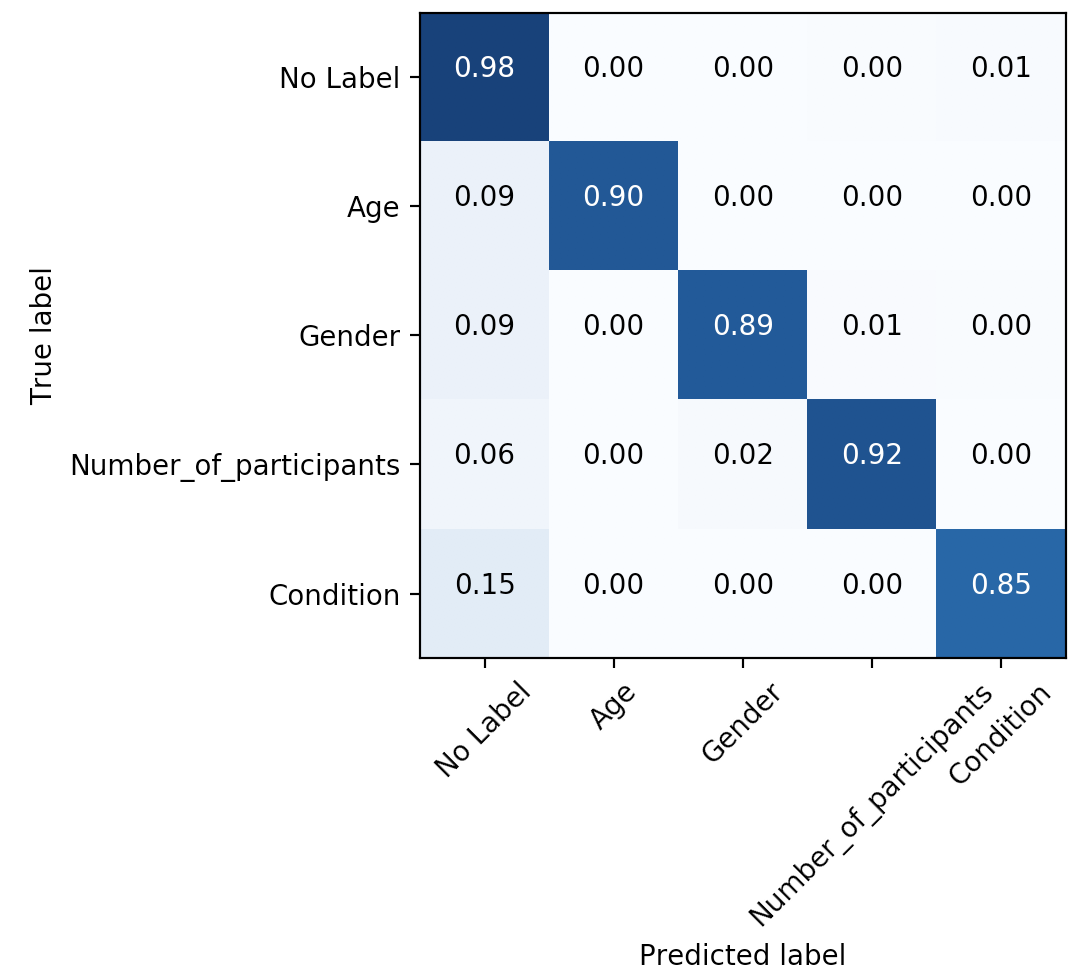
\includegraphics[width=0.35\textwidth]{figs/p_conf_mat.png}
%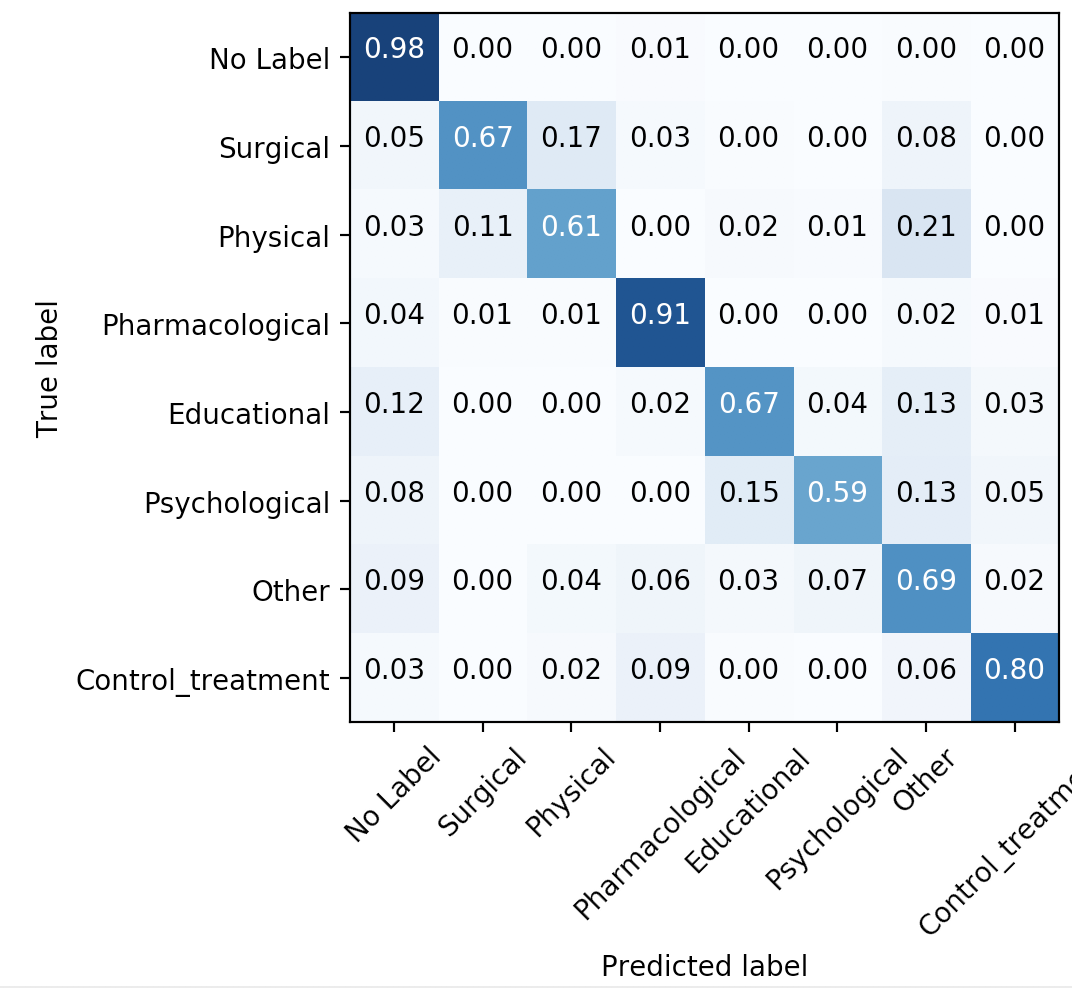
\includegraphics[width=0.35\textwidth]{figs/i_conf_mat.png}
%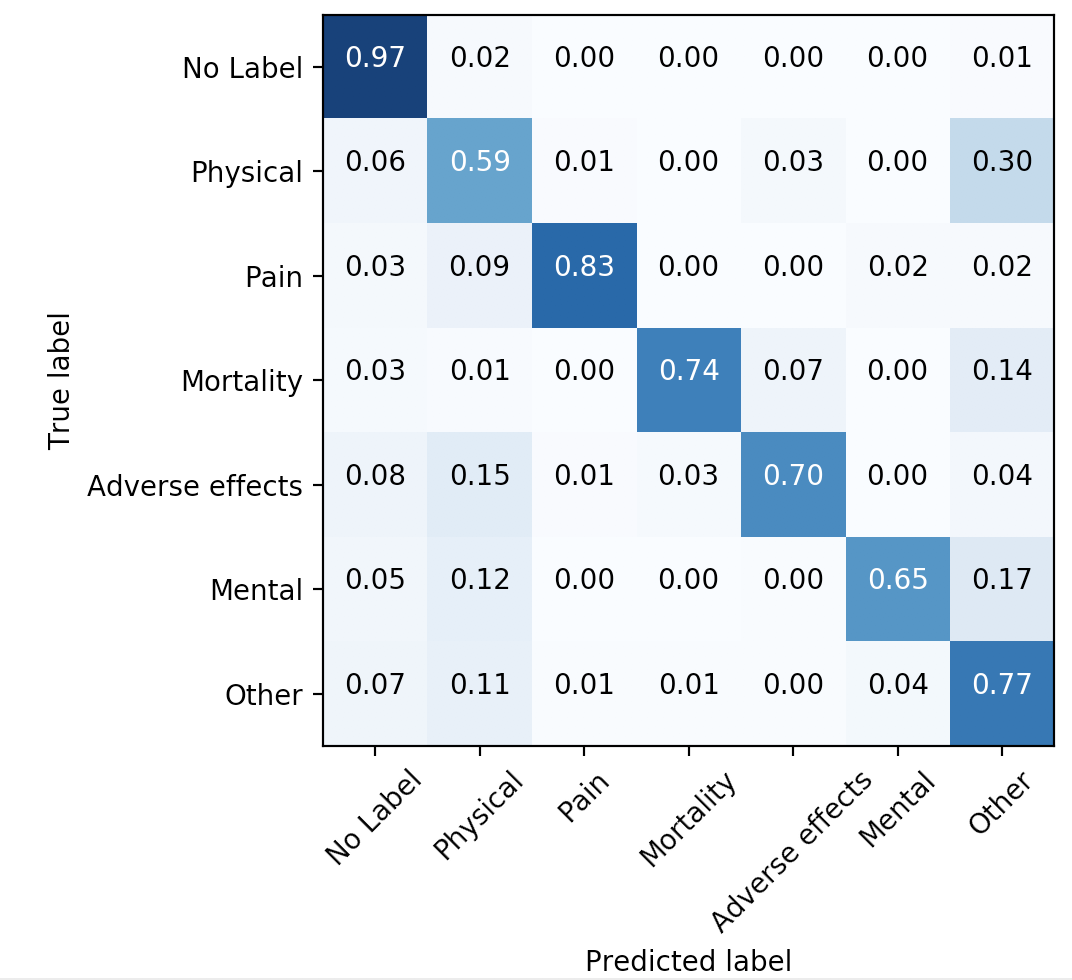
\includegraphics[width=0.35\textwidth]{figs/o_conf_mat.png}
\caption{Confusion matrix for token-level labels provided by experts.}
\label{fig:p_confusion}
\end{figure}

In a similar though more benign category of error, workers differed in the amount of context they included surrounding each subspan.
Although the instructions asked workers to highlight minimal subspans, there was variance in what workers considered relevant.

\begin{table}[h]%[!htb]
    \centering
    \small
    \begin{tabular}{ l c c c } 
    	%\hline
        \textbf{} & Precision & Recall & F-1 \\
        \cline{2-4}
        Participants  & 0.39 & 0.71 & 0.50 \\
        Interventions & 0.59 & 0.60 & 0.60 \\ 
        Outcomes      & 0.70 & 0.68 & 0.69 \\ 
        %\hline
    \end{tabular}
    \caption{Statistics for individual AMT annotations evaluated against the aggregated versions, macro-averaged over different labels.}
   	\label{tab:amt_semantic_stats}
\end{table}

%The agreement between AMT workers is again antagonistic to typical statistics, 
For the same reasons mentioned above (little pairwise overlap in annotations, high variance with respect to annotations per worker), quantifying agreement between AMT workers is again difficult using traditional measures. We thus again take as a measure of agreement the precision, recall, and F-1 of the individual annotations against the aggregated labels and present the results in Table~\ref{tab:amt_semantic_stats}.
% bcw 2/22 -- unless you have v. good reason, easier to just let TeX do its thing w/table placement... at least in my experience. 
%\begin{table}%[!htb]
%    \centering
%    \small
%    \label{tab:basic_exp}
%    \begin{tabular}{ l r r r }
%        \hline
%        \noalign{\vskip 1mm}  
%        \textbf{Participants} & Agreement & Freq (AMT) & Freq \\
%        \textsc{total} & 0.82  & 3.59 & 6.25 \\
%        \hline
%        \noalign{\vskip 1mm}  
%        Age &         0.83 & 0.50 & 0.66 \\
%        Gender &      0.68 & 0.36 & 0.34 \\
%        Sample size & 0.92 & 0.84 & 1.55 \\
%        Condition &   0.84 & 1.89 & 3.70 \\
%        \hline
%        \noalign{\vskip 1mm}  
%        \textbf{Interventions} & Agreement & Freq (AMT) & Freq\\ 
%        \textsc{total} & 0.36 & 5.75 & 8.91 \\
%        \hline
%        \noalign{\vskip 1mm}  
%        Physical & 0.20 & 0.66 & 0.64 \\
%        Surgical & 0.49 & 0.34 & 0.81 \\
%        Control & 0.45 & 0.62 & 0.84 \\
%        Drug & 0.48 & 3.17 & 4.94 \\
%        Education & 0.26 & 0.21 & 0.18 \\
%        Mental & 0.23 & 0.40 & 0.45 \\
%        Other & 0.37 & 0.34 & 1.06 \\
%        \hline
%        \noalign{\vskip 1mm}  
%        \textbf{Outcomes} & Agreement & Freq (AMT) & Freq \\
%        \textsc{total} & 0.63 & 6.63 & 8.79 \\
%        \hline
%        \noalign{\vskip 1mm}  
%        Physical       &  0.54 & 3.14 & 2.85 \\
%        Pain           &  0.95 & 0.19 & 0.28 \\
%        Mortality      &  0.84 & 0.25 & 0.31 \\
%        Adverse effects&  0.45 & 0.50 & 0.66 \\
%        Mental         &  0.60 & 0.74 & 0.54 \\
%        Other          &  0.42 & 1.80 & 4.13 \\
%        \hline
%    \end{tabular}
%    \caption{Agreement between AMT and gold-standard labels, and comparison of the per-document frequency of different subspan labels.}
%\end{table}

\begin{table}[h]%[!htb]
    \centering
    \small
    \begin{tabular}{ l c c } 
    	%\hline
        & \multicolumn{2}{l}{\textbf{Span frequency}} \\
        \cline{1-3}
        \textbf{Participants} & AMT & Experts\\
        \textsc{total} & 3.45 & 6.25 \\
        \cline{2-3}
        \noalign{\vskip 1mm}  
        Age & 0.49 & 0.66 \\
        Condition & 1.77 & 3.69 \\
        Gender & 0.36 & 0.34 \\
        Sample Size & 0.83 & 1.55 \\
        \hline
        \noalign{\vskip 1mm}  
        \textbf{Interventions} & AMT & Experts\\ 
        \textsc{total} & 6.11 & 9.31 \\
        \cline{2-3}
        \noalign{\vskip 1mm}  
        Behavioral & 0.22 & 0.37 \\
        Control & 0.83 & 0.94 \\
        Educational & 0.04 & 0.07 \\
        No Label & 0.00 & 0.00 \\
        Other & 0.23 & 1.12 \\
        Pharmacological & 3.37 & 5.19 \\
        Physical & 0.87 & 0.88 \\
        Psychological & 0.29 & 0.19 \\
        Surgical & 0.24 & 0.62 \\
        \hline
        \noalign{\vskip 1mm}  
        \textbf{Outcomes} & AMT & Experts\\
        \textsc{total} & 6.36 & 10.00 \\
        \cline{2-3}
        \noalign{\vskip 1mm}  
        Adverse effects & 0.45 & 0.66 \\
        Mental & 0.69 & 0.79 \\
        Mortality & 0.23 & 0.33 \\
        Other & 1.77 & 3.70 \\
        Pain & 0.18 & 0.27 \\
        Physical & 3.03 & 4.25 \\
        %\hline
    \end{tabular}
    \caption{Average per-document frequency of different label types.}
   	\label{tab:semantic_label_freq}
\end{table}

\subsection{Repetition}
\label{section:corpus-coref}

Medical abstracts often mention the same information in multiple places.
In particular, interventions and outcomes are typically described at the beginning of an abstract when introducing the purpose of the underlying study, and then again when discussing methods and results. It is important to be able to differentiate between novel and reiterated information, especially in cases such as complex interventions, distinct measured outcomes, or multi-armed trials. Merely identifying all occurrences of, for example, a pharmacological intervention leaves ambiguity as to how many distinct interventions were applied.

Workers identified repeated information as follows. After completing detailed labeling of abstract spans, they were asked to group together subspans that were instances of the same information (for example, redundant mentions of a particular drug evaluated as one of the interventions in the trial).
This process produces labels for repetition between short spans of tokens.
Due to the differences in the lengths of annotated subspans discussed in the preceding section, the labels are not naturally comparable between workers without directly modeling the entities contained in each subspan.
The labels assigned by workers produce repetition labels between sets of tokens but a more sophisticated notion of co-reference is required to identify which tokens correctly represent the entity contained in the span, and which tokens are superfluous noise.

% bcw 5/10 an example would be *really* helpful here
As a proxy for formally enumerating these entities, we observe that a large majority of starting spans only contain a single target relevant to the subspan labeling task, and so identifying repetition between the starting spans is sufficient.
For example, consider the starting intervention span \emph{"underwent conventional total knee arthroplasty"}; there is only one intervention in the span but some annotators assigned the \textsc{surgical} label to all five tokens while others opted for only \emph{"total knee arthroplasty."}
By analyzing repetition at the level of the starting spans, we can compute agreement without concern for the confounds of slight misalignments or differences in length of the subspans.

Overall agreement between AMT workers for span-level repetition, measured by computing precision and recall against the majority vote for each pair of spans, is reported in Table~\ref{table:coref_acc}.

\begin{table}%[!htb]
    \centering
    \small
    \begin{tabular}{  l c c c  }
    	%\hline
        & Precision & Recall & F-1 \\
        \cline{2-4}
        \noalign{\vskip 1mm}  
        Participants & 0.40 & 0.77 & 0.53 \\
        Interventions & 0.63 & 0.90 & 0.74 \\
        Outcomes & 0.47 & 0.73 & 0.57 \\
       	%\hline
    \end{tabular}
    \caption{Comparison against the majority vote for span-level repetition labels.}
    \label{table:coref_acc}
\end{table}

\subsection{MeSH Terms}
\label{section:corpus-mesh}
The National Library of Medicine maintains an extensive hierarchical ontology of medical concepts called Medical Subject Headings (MeSH terms); this is part of the overarching Metathesaurus of the Unified Medical Language System (UMLS).
Personnel at the NLM manually assign citations (article titles, abstracts and meta-data) indexed in MEDLINE relevant MeSH terms. These terms have been used extensively to evaluate the content of articles, and are frequently used to facilitate document retrieval \cite{lu2009evaluation,lowe1994understanding}. 

In the case of randomized controlled trials, MeSH terms provide structured information regarding key aspects of the underlying studies, ranging from participant demographics to methodologies to co-morbidities. A drawback to these annotations, however, is that they are applied at the document (rather than snippet or token) level. To capture where MeSH terms are instantiated within a given abstract text, we provided a list of all terms associated with said article and instructed workers to select the subset of these that applied to each set of token labels that they annotated.

MeSH terms are domain specific and many require a medical background to understand, thus rendering this facet of the annotation process particularly difficult for untrained (lay) workers.
Perhaps surprisingly, several AMT workers voluntarily mentioned relevant background training; our pool of workers included (self-identified) nurses and other trained medical professionals. A few workers with such training stated this background as a reason for their interest in our tasks. % bcw 2/22 -- i think this is true, or i seem to recall seeing emails to this effect, but @ben please verify that I'm not making this up :)
% ben -- indeed! I remember at least two instances and a couple days ago I spent a while searching through my email for the evidence with no success. as long as we both think so I'm confident it's not just wishful thinking

The technical specificity of the more obscure MeSH terms is also exacerbated by their sparsity.
Of the 6,963 unique MeSH terms occurring in our set of abstracts, 87\% of them are only found in 10 documents or fewer and only 2.0\% occur in at least 1\% of the total documents.
The full distribution of document frequency for MeSH terms is show in Figure~\ref{fig:mesh_freq}.

\begin{figure}
\centering
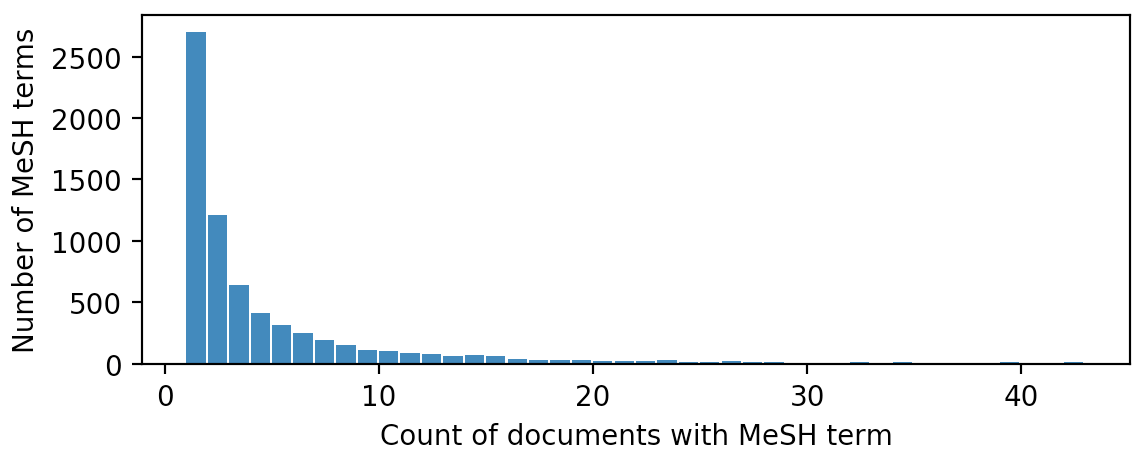
\includegraphics[width=0.475\textwidth]{figs/mesh_freq.png}
\caption{Histogram of the number of documents containing each MeSH term.}
\label{fig:mesh_freq}
\end{figure}

To evaluate how often salient MeSH terms were instantiated in the text by annotators we consider only the 135 MeSH terms that occur in at least 1\% of abstracts (we list these in the supplementary material).
For each term, we calculate its "instantiation frequency" as the percentage of abstracts containing the term in which at least one annotator assigned it to a span of text.
The total numbers of MeSH terms with an instantiation rate above different thresholds for the respective PIO elements are shown in Table~\ref{table:mesh_rates}.

\begin{table}%[!htb]
\small % bcw 5/10 we should be consistent w/table sizing
    \centering
    \begin{tabular}{ l c c c} 
    	\hline
        Inst. Freq & 10\% & 25\% & 50\% \\
        \hline
        Participants & 65 & 24 & 7 \\
        Interventions & 106 & 68 & 32 \\
        Outcomes & 118 & 108 & 75 \\
        \hline
    \end{tabular}
    \caption{The number of common MeSH terms (out of 135) that were assigned to a span of text in at least 10\%, 25\%, and 50\% of the possible documents. } % bcw 2/22 -- not totally clear to me what is meant here by 'minimum frequencies'?
    	\label{table:mesh_rates}
\end{table}

\section{Tasks \& Baselines}
\label{section:tasks-baselines}

We outline a few NLP tasks that are central to the aim of processing medical literature generally and to aiding practitioners of EBM specifically. First, we consider the task of identifying spans in abstracts that describe the respective PICO elements (Section \ref{section:tasks-spans}). This would, e.g., improve medical literature search and retrieval systems. Next, we outline the problem of extracting structured information from abstracts (Section \ref{section:tasks-extraction}). Such models would further aid search, and might eventually facilitate automated knowledge-base construction for the clinical trials literature. Furthermore, automatic extraction of structured data would enable automation of the manual evidence synthesis process \cite{marshall:2017:ACL}.

Finally, we consider the challenging task of identifying redundant mentions of the same PICO element (Section \ref{section:tasks-repetition}). This happens, e.g., when an intervention is mentioned by the authors repeatedly in an abstract, potentially with different terms. Achieving such disambiguation is important for systems aiming to induce structured representations of trials and their results, as this would require recognizing and normalizing the unique interventions and outcomes studied in a trial.  

%, which would expedite data extraction

%, thus enabling semi- or even (eventually) full automation of the manual evidence synthesis process (Section \ref{section:tasks-extraction}).  


%The corpus presented in this work facilitates empirical work on these tasks at a scale not currently possible. 

For each of these tasks we present baseline models and corresponding results. Note that we have pre-defined train, development and test sets across PIO elements for this corpus, comprising 4300, 500 and 200 abstracts, respectively. The latter set is annotated by domain experts (i.e., persons with medical training). These splits will, of course, be distributed along with the dataset to facilitate model comparisons.
% bcw 2/22 TODO TODO TODO I am leaving the above numbers for now/submission, but IF THIS GETS ACCEPTED WE NEED TO MAKE SURE THIS IS ACCURATE; currently we have 200 in test set only for semantic annotations! hopefully we can acquire rest before camera ready. also for some reason Yinfei had used a 3456 split for train set, but i can't recall why... 
% bcw 5/10 -- TODO! get the above numbers right (precisely!) -- note exactly 5k in total i don't think... 

%central to the efforts of evidenced based medicine experts and corresponding baselines.

\subsection{Identifying P, I and O Spans}
\label{section:tasks-spans}

We consider two baseline models: a linear Conditional Random Field (CRF) ~\cite{lafferty2001conditional} and a Long Short-Term Memory (LSTM) neural tagging model, an LSTM-CRF \cite{lample2016neural,ma-hovy:2016:P16-1}. In both models, we treat tokens as being either Inside (I) or Outside (O) of spans.  % Both models take as input a sentence with tags indicating the PICO element for each word.

% bcw 2/21 -- in general suggest avoiding using 'etc.' in  "scientific" writing, but opinions probably vary on this !
% bcw 2/21 -- 
For the CRF, features include: indicators for the current, previous and next words; part of speech tags inferred using the Stanford CoreNLP tagger \cite{DBLP:conf/acl/ManningSBFBM14}; and character information, e.g., whether a token contains digits, uppercase letters, symbols and so on.% 
% bcw 2/22 -- where did the POS tags come from? we should specify
% roma -- StanfordCoreNLP
% bcw 2/22 -- moved the IO bit up here, but we do use this for both variants, right?
% roma -- yes, same tagging scheme!

%3 individual models:
%\begin{table}%[!htb]
%\small
%\centering
%\begin{tabular}{ c c c c c}
%\hline
%\bf{CRF} & Precision & Recall & F-1 \\
%\hline
%Participants & 70.29 & 38.75 & 49.95 \\
%Interventions & 47.01 & 43.89 & 45.39 \\
%Outcomes & 64.78 & 10.47 & 18.02 \\
%\hline
%\bf{LSTM-CRF} & Precision & Recall & F-1 \\
%\hline
%Participants & 62.27 & 49.48 & 55.14 \\
%Interventions & 52.37 & 40.49 & 45.67 \\
%Outcomes & 47.91 & 36.16 & 41.21 \\
%\hline
%\end{tabular}
%\caption{Performances of baseline CRF and LSTM-CRF models on the PIO span tagging task.}
%\end{table}

%one multi-task model that tags as P, I, O or N
\begin{table}%[!htb]
\small
\centering
\begin{tabular}{ l c c c c}
\hline
\bf{CRF} & Precision & Recall & F-1 \\
\cline{2-4}
Participants & 0.55 & 0.51 & 0.53 \\
Interventions & 0.65 & 0.21 & 0.32 \\
Outcomes & 0.83&0.17&0.29\\
\hline
\bf{LSTM-CRF} & Precision & Recall & F-1 \\
\cline{2-4}
Participants & 0.78&0.66&0.71 \\
Interventions & 0.61&0.70&0.65 \\
Outcomes & 0.69&0.58&0.63 \\
\hline
\end{tabular}
\caption{Baseline models (on the test set) for the PIO span tagging task.}
\end{table}
For the neural model, the model induces features via a bi-directional LSTM that consumes distributed vector representations of input tokens sequentially. The bi-LSTM yields a hidden vector at each token index, which is then passed to a CRF layer for prediction. We also exploit character-level information by passing a bi-LSTM over the characters comprising each word ~\cite{lample2016neural}; these are appended to the word embedding representations before being passed through the bi-LSTM. % bcw 2/22 -- i assume appended to the word representations? or is it the hidden layer they're appended to?
% roma -- appended to the word, yes!

% bcw 2/22 -- do we fine-tune the vectors or just use as static inputs??
% roma -- we're using non-static!

%  -- also, which layer is the dropout used?? and just one?
% roma -- dropout is on input of LSTM

%  -- how do we initialize the char embeddings? what is their dimension?
% roma -- char embeddings are 100 dimensional (didn't experiment with different dimension size), they're initialised randomly and trained over data before the LSTM process!

%To initialize word vectors we use 200 dimensional embeddings pre-trained over 5.5 billion words from medical articles  ~\cite{moen2013distributional} (these are fine-tuned during training). Character embeddings are 100 dimensional and initialized randomly. We set the hidden state dimensionality for the LSTM to 200, and set dropout on the output layer of the LSTM to 0.5. For parameter estimation we use the Adam optimizer with a learning rate of 0.001. 

\subsection{Extracting Structured Information}
\label{section:tasks-extraction}
% bcw 2/22 -- this is not clear at all - what are we predicting???

Beyond identifying the spans of text containing information pertinent to each of the PIO elements, we consider the task of predicting which of the detailed labels occur in each span, and where they are located.
Specifically, we begin with the starting spans and predict a single label from the corresponding PIO hierarchy for each token, evaluating against the test set of 200 documents.
Initial experiments with neural models proved unfruitful but bear further investigation.

For the CRF model we include the same features as in the previous model, supplemented with additional features encoding if the adjacent tokens include any parenthesis or mathematical operators (specifically: $\%, +, -$).
For the logistic regression model, we use a one-vs-rest approach.
Features include token $n$-grams, part of speech indicators, and the same character-level information as in the CRF model. 

\begin{table}%[!htb]
\small
    \centering
    \begin{tabular}{ l c c c} 
    	\hline
        \textbf{LogReg} & Precision & Recall & F-1 \\
        \cline{2-4}
        Participants & 0.41 & 0.20 & 0.26 \\
        Interventions & 0.79 & 0.44 & 0.57 \\
        Outcomes & 0.24 & 0.21 & 0.22 \\
        \hline
        \textbf{CRF} & Precision & Recall & F-1 \\
        \cline{2-4}
        Participants & 0.41 & 0.25 & 0.31 \\
        Interventions & 0.59 & 0.15 & 0.21 \\
        Outcomes & 0.60 & 0.51 & 0.55\\
       	\hline
    \end{tabular}
    \caption{Baseline models for the token-level, detailed labeling task.}
\end{table}

\subsection{Detecting Repetition}
\label{section:tasks-repetition}

To formalize repetition, we consider every pair of starting PIO spans from each abstract, and assign binary labels that indicate whether they share at least one instance of the same information.
Although this makes prediction easier for long and information-dense spans, a large enough majority of the spans contain only a single instance of relevant information that the task serves as a reasonable baseline.
Again, the model is trained on the aggregated labels collected from AMT and evaluated against the high-quality test set. % bcw 2/22 -- perhaps revisit here
% bcw 2/22 @Ben why are we evaluating on the train and not the test???

We train a logistic regression model that operates over standard features, including bag-of-words representations and sentence-level features such as length and position in the document. All baseline model implementations are available on the corpus website. % bcw 5/11 -- need to make sure this is true!!

\begin{table}%[!htb]
\small
    \centering
    \begin{tabular}{ l c c c} 
    	%\hline
        \textbf{} & Precision & Recall & F-1 \\
        \cline{2-4}
        \noalign{\vskip 1mm}  
        Participants & 0.39 & 0.52 & 0.44 \\
        Interventions & 0.41 & 0.50 & 0.45 \\
        Outcomes & 0.10 & 0.16 & 0.12 \\
        %\hline
	\end{tabular}
    \caption{Baseline model for predicting whether pairs of spans contain redundant information.}%, assessed on the test set.} % bcw -- apparently not on the test set??? we will need to explain this
\end{table}

\section{Conclusions}
\label{section:conclusions}

We have presented EBM-NLP: a new, publicly available corpus comprising 5,000 richly annotated abstracts of articles describing clinical randomized controlled trials. This dataset fills a need for larger scale corpora to facilitate research on NLP methods for processing the biomedical literature, which have the potential to aid the conduct of EBM. The need for such technologies will only become more pressing as the literature continues its torrential growth.  

The EBM-NLP corpus, accompanying documentation, code for working with the data, and baseline models presented in this work are all publicly available at: \url{http://www.ccs.neu.edu/home/bennye/EBM-NLP}. % bcw 5/10, again not totally married to using this URL, but we need somethign!


\section{Acknowledgements}

This work was supported in part by the National
Cancer Institute (NCI) of the National Institutes of
Health (NIH), award number UH2CA203711. 
%%%% oops... we forget to ack the NIH (sigh). let's put here and in arxiv version... maybe we can even ask ACL folks if we're not too late to include...


% will all be made publicly available upon publication. 

% bcw: 2/20 -- (1) this will eventually be moved to a separate doc. (2) we should also include all instruction PDFs. Basically, this is going to be a very large appendix.

% bcw 2/22 -- moved to https://www.overleaf.com/13969921zhhqnsygwndy#
% might want some of these back in if we have the space anyway, though
\begin{comment}
\clearpage

\section{Corpus Details: Appendix}

\subsection{PIO: Participants}
In the Participants task, we sought primarily to capture the specific characterizations of the population that would affect treatment decisions or inclusion/exclusion criteria in systematic reviews.
The starting spans for the participants were often a full sentence in length, describing the relevant demographic information of the subjects.
The targeted information and hierarchy of labels are depicted in Figure~\ref{p_labels}.

The available ranges for the Age label were derived from combining the age-specific MeSH terms into higher level categories.
For example, the \textsc{[Young]} category covers the MeSH terms for \textsc{[Infant, Newborn]}, \textsc{[Infant]}, \textsc{[Child, Preschool]} and \textsc{[Child]}.

\begin{figure}
\small
\label{p_labels}
\begin{tikzpicture}[%
  grow via three points={one child at (0.5,-0.7) and
  two children at (0.5,-0.7) and (0.5,-1.4)},
  edge from parent path={(\tikzparentnode.south) |- (\tikzchildnode.west)}]
    \node {Participants}
    child { node {Gender}
    	child { node{Male}}
        child { node{Female}}
    }		
    child [missing] {}
    child [missing] {}
    child { node {Age}
      child { node{Young [0-12]}}
      child { node{Adolescent [13-18]}}
      child { node{Adult [19-64]}}
      child { node{Aged [65+]}}
    }
    child [missing] {}
    child [missing] {}
    child [missing] {}
    child [missing] {}
    child { node {Number of Participants}
      child { node {All Enrolled Participants}}
      child { node {Subgroup of Participants}}
    }
    child [missing] {}				
    child [missing] {}				
    child { node {Condition}
      child { node {Disease}}
      child { node {Other Characteristic}}
    };
\end{tikzpicture}
\caption{Participant task label hierarchy}
\end{figure}

\subsection{PIO: Interventions}

For the intervention task, the starting spans were almost always short and contained only the specific intervention used in the trial and therefore the task focused less on anchoring specific types of information in the text and more on assigning the intervention type and semantic labels.
The intervention types chosen for this task are the subset of the the labels provided by a domain expert (TODO: where did Iain get these labels) that remain after removing overly technical and rare categories.

To compliment the MeSH terms from the article, we provide two additional semantic labels: \textsc{Complex} to indicate when the intervention was applied in conjunction with at least one other intervention, and \textsc{Dosage Change} for cases where the same intervention is repeated but at different dosages.

% bcw 12/14: these are nice, but take up a lot of room, will probably want to reduce size or maybe just have one an put others in supplemental material/appendix doc. also, would be prettier in Omnigraffle :) we can buy for you if you want
% bcw 2/20: have switched to 'small' and prettified a tad, or tried to... 
\begin{figure}
\small
\label{i_labels}
\begin{tikzpicture}[%
  grow via three points={one child at (0.5,-0.7) and
  two children at (0.5,-0.7) and (0.5,-1.4)},
  edge from parent path={(\tikzparentnode.south) |- (\tikzchildnode.west)}]
  \node {Interventions}
    child { node {Physical}
      child { node {Surgical}}
      child { node {Pharmacological}}
    }
    child [missing] {}
    child [missing] {}
    child { node {Non-physical}
      child { node{Educational}}
      child { node{Behavioral}}
      child { node{Psychological}}
    }
    child [missing] {}
    child [missing] {}
    child [missing] {}
    child { node {No Active Treatment}};
\end{tikzpicture}
\caption{Intervention task label hierarchy}
\end{figure}

\subsection{PIO: Outcomes}

The labels for the outcomes task shown in Figure~\ref{o_labels} are derived from the vocabulary used by the Cochrane Collection \citep{davey2011characteristics}, adjusted to remove rare categories and better capture the types of spans observed in the initial dataset.

A common occurrence in the discussion of outcomes is to provide a general description of the outcome (e.g. "average pain"), and then later go in to more detail about the way the measurement was taken (e.g. "pain score on a visual analog scale from 0-10").
To capture this relationship we provided the annotators with the ability to select if any particular outcome is \textsc{General} or \textsc{Specific}, and instructed them to mark any outcomes differing only in their level of specificity as co-referent.

\begin{figure}
\small
\label{o_labels}
\begin{tikzpicture}[%
  grow via three points={one child at (0.5,-0.7) and
  two children at (0.5,-0.7) and (0.5,-1.4)},
  edge from parent path={(\tikzparentnode.south) |- (\tikzchildnode.west)}]
  \node {Outcomes}
    child { node {Physical Health}
    	child { node{Pain}}
    	child { node{Adverse Effects}}
    	child { node{Mortality}}
    }		
    child [missing] {}
    child [missing] {}
    child [missing] {}
    child { node {Mental/Behavioral Impact}
      child { node{Mental Health}}
      child { node{Participant Behavior}}
      child { node{Satisfaction With Care}}
    }
    child [missing] {}
    child [missing] {}
    child [missing] {}
    child { node {Non-health Outcome}
      child { node {Quality of Intervention}}
      child { node {Resource Use}}
      child { node {Withdrawals from Study}}
    };
\end{tikzpicture}
\caption{Outcome task label hierarchy}
\end{figure}


A recurring issue with aggregation across noisy labels is the necessity of handling low quality workers.
Due to the high variance of worker skill levels on mechanical turk, even filtering workers leaves some disparity in the quality of annotations.
Using models that encode worker reliability is therefore highly desirable, and evaluation of results is best done with this aspect in mind as well.

One saving grace is that prolific workers tend to fall in to two categories: spammers submitting low quality work which is easily detected and disregarded, and those with an aptitude or interest for the work.

\begin{figure}
\centering
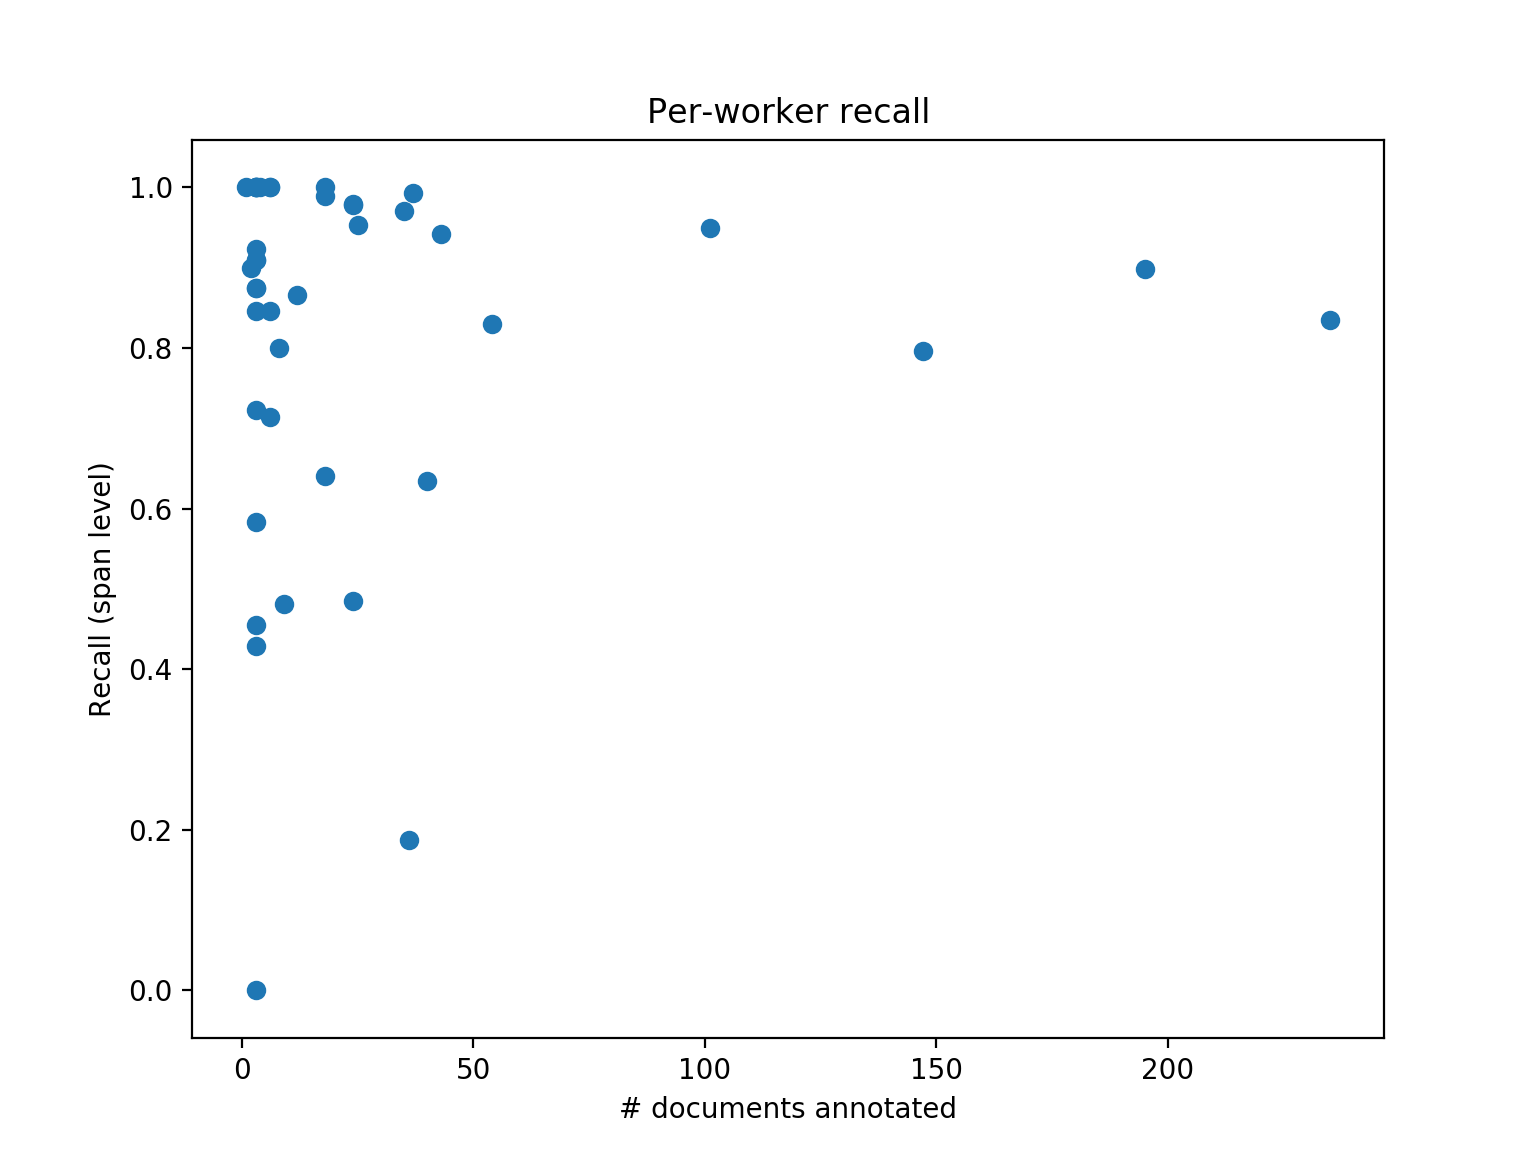
\includegraphics[width=0.4\textwidth]{figs/worker_span_recall.png}
\caption{Span level recall of workers vs. how many documents they annotated (on P).}
\end{figure}

\subsection{MeSH terms in at least 1\% of documents}
Humans, Female, Male, Adult, Middle Aged, Aged, Double-Blind Method, Treatment Outcome, Adolescent, Prospective Studies, Child, Follow-Up Studies, Time Factors, Child Preschool, Aged 80 and over, Young Adult, Autistic Disorder, Cross-Over Studies, Dose-Response Relationship Drug, Drug Therapy Combination, Clinical Trials as Topic, Random Allocation, Drug Administration Schedule, Blood Pressure, Antineoplastic Combined Chemotherapy Protocols, Risk Factors, Analysis of Variance, Questionnaires, Combined Modality Therapy, Infant, Placebos, Administration Oral, Hypertension, Postoperative Complications, Pain Measurement, Single-Blind Method, Quality of Life, Pilot Projects, Pregnancy, Severity of Illness Index, Animals, Child Development Disorders Pervasive, Prognosis, Breast Neoplasms, Psychiatric Status Rating Scales, Heart Rate, Infusions Intravenous, Survival Rate, Antineoplastic Agents, Pain Postoperative, Infant Newborn, Survival Analysis, Acute Disease, Patient Satisfaction, Recurrence, Neoplasm Staging, Chronic Disease, Blood Glucose, Disease-Free Survival, Drug Combinations, Myocardial Infarction, Hemodynamics, Fluorouracil, Age Factors, Pain, Chi-Square Distribution, Injections Intravenous, Anti-Bacterial Agents, Patient Compliance, Exercise, Cyclophosphamide, Patient Education as Topic, Statistics Nonparametric, Antipsychotic Agents, Heart Failure, Recombinant Proteins, Antihypertensive Agents, Social Behavior, Biological Markers, Neoplasms, United States, Attention, Incidence, Neoplasm Recurrence Local, Neuropsychological Tests, Reproducibility of Results, Reference Values, Research Design, Doxorubicin, Dietary Supplements, Disease Progression, Insulin, Risk Assessment, Exercise Therapy, Body Mass Index, Sensitivity and Specificity, Lung Neoplasms, Randomized Controlled Trials as Topic, Retrospective Studies, Diabetes Mellitus Type 2, Anesthetics Local, Behavior Therapy, Electrocardiography, Body Weight, Asthma, Psychomotor Performance, Anti-Inflammatory Agents Non-Steroidal, Cognitive Therapy, Coronary Disease, Length of Stay, Exercise Test, Methotrexate, Risperidone, Obesity, Administration Topical, Parents, Reaction Time, Aspirin, Muscle Skeletal, Proportional Hazards Models, Cisplatin, Longitudinal Studies, Lipids, Prostatic Neoplasms, Chemotherapy Adjuvant, Equipment Design, Regression Analysis, Diet, Cost-Benefit Analysis, Adenocarcinoma, Communication, Neoplasm Metastasis, Area Under Curve, Cognition, Activities of Daily Living


%\sub

% bcw 12/14 : suggest making this a key section -- what do we view as the important tasks on this, and what are reasonable baselines
\subsection{Other Properties}
\subsubsection{Label distribution}
Relative label frequencies, per-document uses

\begin{figure}
\centering
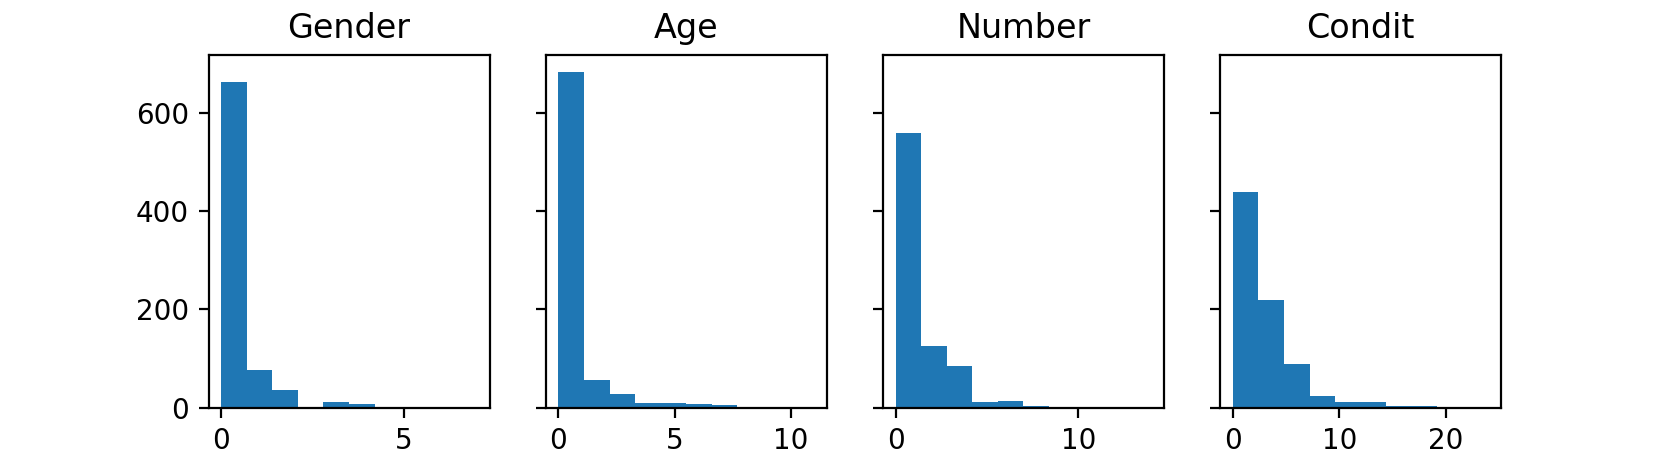
\includegraphics[width=0.4\textwidth]{figs/nsubspans_per_doc_hist.png}
\caption{How many times is each label used per document? (for P).}
\end{figure}
\end{comment}

%\clearpage
\bibliography{acl2018}
\bibliographystyle{acl_natbib}

\end{document}


\section{Applications and Future Work}

% include your own bib file like this:
%\bibliographystyle{acl}

\bibliography{acl2018}
\bibliographystyle{acl_natbib}

\appendix

\section{Multiple Appendices}
\dots can be gotten by using more than one section. We hope you won't
need that.

\end{document}
